\originalchapter{一般重整化、子图与局域性}
\label{ch:general-renormalization}

一圈计算告诉我们怎样确定反项,却还没有回答高阶图是否要求新的、任意多的参数.特别是,一个图在所有环动量共同变大时可能收敛,但在只有某个环动量变大时仍会发散.本章先区分这两种问题,再说明为什么局域反项能逐阶解决它们.所使用的全阶收敛定理会明确陈述其范围;我们会完整展开一个两圈例子的减除结构,而不把例子冒充全阶定理的证明.

\originalsection{表面发散次数}

对一个连通费曼图,把各独立环动量同时缩放为 $k_a\mapsto sk_a$.计入积分测度后,若径向积分的大 $s$ 行为为 $\int^\Lambda s^{D-1}\dd s$,则称 $D$ 为表面发散次数.$D>0$ 对应可能的幂次发散,$D=0$ 对应可能的对数发散.这里的“可能”有两层含义:对称性可使最高次项抵消;另一方面,$D<0$ 只检查了共同缩放,尚未排除子图发散.

以四维 QED 为例,令 $I_A,I_\psi$ 是内部光子、电子线数,$E_A,E_\psi$ 是外腿数,$V$ 是三点顶角数.光子传播子大动量按 $k^{-2}$ 衰减,电子传播子含一个分子动量而按 $k^{-1}$ 衰减,故
\begin{equation}
 D=4L-2I_A-I_\psi.
\end{equation}
图的拓扑恒等式为
\begin{equation}
 2I_A+E_A=V,\qquad 2I_\psi+E_\psi=2V,\qquad
 L=I_A+I_\psi-V+1.
\end{equation}
消去内部结构便得到
\begin{equation}
 D=4-E_A-\frac32E_\psi.
 \label{eq:qed-superficial-degree}
\end{equation}
它不含 $V$,因而无论微扰阶数多高,可能整体发散的外腿类型只有有限种.例如 $E_\psi=2,E_A=2$ 给 $D=-1$,但在电子线上插入自能子图后,振幅仍包含那个子图的发散.必须对每个子图分别应用计数.

一般理论也有同样的形式.令场种类为 $\phi_f$,其自由动能决定的工程维数为 $\Delta_f$;第 $i$ 类顶角有 $n_i$ 个导数、$n_{if}$ 个 $\phi_f$,耦合为 $g_i$.作用量无量纲,因此
\begin{equation}
 [g_i]\equiv\delta_i=d-n_i-\sum_f n_{if}\Delta_f.
\end{equation}
截肢的 $\{E_f\}$ 点核有量纲 $d-\sum_fE_f\Delta_f$.一个具有 $V_i$ 个第 $i$ 类顶角的图已带 $\prod_i g_i^{V_i}$,余下动量积分的次数于是为
\begin{equation}
 D=d-\sum_fE_f\Delta_f-\sum_iV_i\delta_i.
 \label{eq:general-superficial-degree}
\end{equation}
也可以由 $L=I-V+1$ 和每种场的端点计数导出它.这个论证假定局域顶角和通常的二阶玻色、一次费米动能;含高导数传播子的理论要先重新确定大动量衰减,不能无条件套用.

若所有 $\delta_i>0$,增加顶角数会降低 $D$,通常只有有限多个发散图,这类理论称为超可重整.若所有 $\delta_i\geq0$,且场的工程维数为正,发散外腿类型只有有限多,称为幂计数可重整.若存在 $\delta_i<0$,增加该类顶角可能不断提高 $D$,通常要引入无穷多个算符,称为幂计数不可重整.维数零的场、特殊对称性、拓扑理论以及强耦合固定点,需要比这段通常的幂计数更细的分析.

\begin{example}
在四维比较 $\phi^3$、$\phi^4$、$\phi^6$ 三种标量相互作用.
\end{example}
\begin{solution}
动能 $\tfrac12(\partial\phi)^2$ 给 $[\phi]=1$,所以 $[g_3]=1$,$[\lambda]=0$,$[g_6]=-2$.对纯 $\phi^n$ 图,\eqref{eq:general-superficial-degree} 成为
$D=4-E-(4-n)V$.
$\phi^3$ 每增加一个顶角就降低一次 $D$;$\phi^4$ 的 $D=4-E$ 不随阶数变化;$\phi^6$ 则有 $D=4-E+2V$,高阶可产生含更多外腿和导数的发散.这不是说 $\phi^6$ 不能使用,而是说不能仅靠一个 $g_6$ 在任意能量、任意阶数保持预测.
\end{solution}

\originalsection{发散部分为什么对应局域反项}

暂设一个图没有发散真子图,并用非零质量避免零动量处的红外问题.其积分核中的传播子形如 $[(k+p)^2+m^2]^{-1}$.对外动量求导,出现
\begin{equation}
 \frac{\partial}{\partial p_\mu}\frac1{(k+p)^2+m^2}
 =-\frac{2(k+p)_\mu}{[(k+p)^2+m^2]^2},
\end{equation}
所以共同缩放的次数至少降低一.对所有外动量作总阶数 $D+1$ 的导数后,整体紫外积分收敛.故发散只能在外动量总次数不超过 $D$ 的多项式中:
\begin{equation}
 M(p_1,\ldots,p_E)
 =\sum_{|\alpha|\leq D}c_\alpha p^\alpha+M_{\rm finite}(p_1,\ldots,p_E).
 \label{eq:local-divergent-polynomial}
\end{equation}
这里 $\alpha$ 是多重指标,还要匹配洛伦兹、自旋和内部群指标.动量空间中的 $p^\alpha$ Fourier 变换为同一点处的导数,因而恰好由局域算符
$c_\alpha\partial^\alpha\prod_f\phi_f^{E_f}$ 产生.非多项式的对数或阈值函数可以出现在有限部分中,却不能作为新的非局域紫外反项.

上述论证的限制也非常重要.对整体外动量求导不一定影响一个内部发散子图;因此必须先把子图发散减掉,才能用它判断整体发散部分的局域性.严格的收敛分析还需要检查所有环动量子空间,而不是只检查一条共同缩放路径.

\originalsection{QED 中全部可能的反项}

结合 \eqref{eq:qed-superficial-degree} 与对称性,可以逐项列出需要检查的类型.
没有外腿的真空图有 $D=4$,对应常数反项;在固定平直时空中,它只改变真空归一化.在有引力时,真空能与宇宙学常数相关,不能再当作无物理意义的整体常数.
奇数费米子外腿的核因费米子数与 Lorentz 结构消失.光子一点评价在 Lorentz 不变真空中也为零.两光子核表面上 $D=2$,允许 $g^{\mu\nu}$、$q^2g^{\mu\nu}$、$q^\mu q^\nu$;Ward 恒等式却只保留 $(q^2g^{\mu\nu}-q^\mu q^\nu)C$.因此只需要 $F_{\mu\nu}F^{\mu\nu}$,不允许独立的 $A_\mu A^\mu$ 质量反项.

三光子图由电荷共轭消失.原因是 $A_\mu$ 与电磁流在电荷共轭下都变号,而真空和作用量保持不变;奇数个此类算符的真空期望等于其负值.这是 Furry 定理的对称性解释.四光子核有 $D=0$,潜在发散只能是不含外动量的常数四阶张量;对每个光子施加 Ward 收缩后,这个常数必须为零.也就是说,单个排序的电子盒图可有表面发散,但全部允许排序的和不需要 $A^4$ 反项.

电子二点核有 $D=1$,其发散为 $a\slashed p+bm$,由电子动能与质量反项吸收.电子电子光子核有 $D=0$,发散为 $c\gamma^\mu$,由电磁顶角反项吸收,且 Ward 恒等式给 $Z_1=Z_2$.除真空常数外,这正是前章列出的反项.图的阶数改变系数,不改变所需算符类型.

这也提供一种更有效的建模原则:先列出全部满足指定对称性且维数不超过四的局域算符,不能仅保留自己最初喜欢的几个项.若某个允许算符的系数在某一阶恰好为零,也不能仅凭这一阶声称它永远不出现.对非 Abel 规范理论,保证这一闭合结构的是规范固定后的 BRST 恒等式;一般的动量截断若破坏对称性,需要相容的恢复步骤.

\originalsection{子图、森林与两圈重叠发散}

一个紫外发散子图 $\gamma$ 的外腿包括连到其余图的内部线;这些腿的动量对 $\gamma$ 而言必须当作外动量.将 $\gamma$ 的发散多项式替换成一个反项顶角,记为把子图收缩得到的图 $G/\gamma$.例如电子自能子图可换成二点反项,顶角子图可换成三点反项.对彼此分离的子图,可以同时收缩;对子图内部还含子图的情形,必须从内向外减除.

困难在于两个发散子图共享内部线,却互不包含.它们不能同时当作独立因子减除,否则会重复减去不存在的区域.为描述这个限制,引入森林:一个森林是由若干发散真子图组成的集合,其中任意两个子图彼此不相交,或者一个包含另一个.互相重叠而不包含的两个子图,不能同属于一个森林.

在有质量标量理论中,令 $t_\gamma^{D_\gamma}$ 表示对子图外动量在零点作总阶数 $D_\gamma$ 的 Taylor 多项式.对真子图先执行森林减除,记为 $\overline R G$,最后减去整体 Taylor 多项式:
\begin{equation}
 \overline R G=\sum_{F\in\mathfrak F(G)}
       \left(\prod_{\gamma\in F}-t_\gamma^{D_\gamma}\right)G,
 \qquad RG=(1-t_G^{D_G})\overline R G.
 \label{eq:bphz-forest-formula}
\end{equation}
空森林给原图;嵌套子图的算符按从内向外的顺序作用.Taylor 算符在积分核上操作,不能先把发散积分算成一个无穷数再相减.对于无质量理论,零动量减除可能制造红外发散,需要非例外减除点或专门的红外处理.

\begin{example}
考察有质量四维 $\lambda\phi^4/4!$ 理论的两圈二点夕阳图.写出它的三个重叠子图及减除结构.
\end{example}
\begin{solution}
在 Euclidean 动量中,取 $m^2>0$,并将四次耦合写为 $\mu^\epsilon\lambda$,使 $d=4-\epsilon$ 中的 $\lambda$ 无量纲.去掉整体 Minkowski 因子后图的积分为
\begin{equation}
 I_G(p)=\frac{\lambda^2\mu^{2\epsilon}}{6}\int\frac{\dd^dk\,\dd^dq}{(2\pi)^{2d}}
 \frac1{(k^2+m^2)(q^2+m^2)[(p-k-q)^2+m^2]}.
 \label{eq:sunset-two-loop-integral}
\end{equation}
$1/6$ 是两顶角、三条相同内部线的对称因子.整体有 $L=2,I=3$,所以 $D_G=2d-6=2$ 在 $d=4$ 时成立.任选三条线中的两条,连同两个顶角,都是一圈四点泡图;它有四条外腿、$D_\gamma=0$.于是共有 $\gamma_1,\gamma_2,\gamma_3$ 三个对数发散子图,任意两个共享一条内部线,互不包含.

\begin{center}
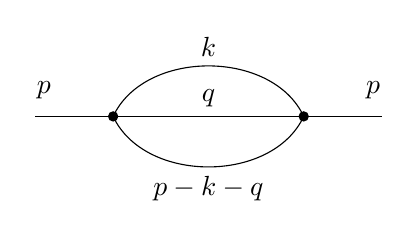
\begin{tikzpicture}[scale=1.1]
 \coordinate (L) at (-1.1,0);\coordinate (R) at (1.1,0);
 \draw (-2,0)--(L);\draw (R)--(2,0);
 \draw (L) to[bend left=65] node[above] {$k$} (R);
 \draw (L)--node[above] {$q$}(R);
 \draw (L) to[bend right=65] node[below] {$p-k-q$} (R);
 \fill (L) circle(1.7pt);\fill (R) circle(1.7pt);
 \node at (-1.9,.3) {$p$};\node at (1.9,.3) {$p$};
\end{tikzpicture}
\end{center}

因此允许的真子图森林只有空集和三个单元素集合,给出
\begin{equation}
 RG=(1-t_p^2)\left[G-t_{\gamma_1}^0G
                       -t_{\gamma_2}^0G-t_{\gamma_3}^0G\right].
 \label{eq:sunset-forest}
\end{equation}
不存在 $t_{\gamma_i}t_{\gamma_j}G$ 的交叉项.这个缺失正是重叠子图与彼此分离子图的区别.

可以对 $\gamma_1$ 直接复算.把它选为携带 $q$ 与 $p-k-q$ 的两条线,其总外动量为 $P=p-k$.泡图是
\begin{align}
 B(P)&=\mu^\epsilon\int\frac{\dd^dq}{(2\pi)^d}
       \frac1{(q^2+m^2)[(P-q)^2+m^2]},\notag\\
 B(P)-B(0)&=-\frac1{16\pi^2}\int_0^1\dd x\,
       \log\left[1+\frac{x(1-x)P^2}{m^2}\right]+\order(\epsilon).
 \label{eq:sunset-bubble-subtraction}
\end{align}
两项分别含 $2/\epsilon$ 极点,它们的差没有极点;这说明反项确实只依赖局域常数.$t_{\gamma_1}^0G$ 的环核为
$[(k^2+m^2)(q^2+m^2)^2]^{-1}$,也就是 $B(0)$ 乘余下的蝌蚪积分.其他两个子图经重新选环动量有相同结构.收缩后的蝌蚪仍有整体发散,需要 $1-t_p^2$ 所对应的二阶二点反项.整体反项只能是 $a+bp^2$,因此只修正质量和动能.

为了进一步检查两个环的共同紫外区,可用 Schwinger 参数.将三条分母各写成 $\int_0^\infty\dd a\,\e^{-a(k^2+m^2)}$;二重高斯积分产生 $U^{-d/2}$,其中 $U=ab+ac+bc$.令 $a,b,c=s(\alpha,\beta,\gamma)$,$\alpha+\beta+\gamma=1$,积分 $s$ 后得
\begin{equation}
 I_G(p)=\frac{\lambda^2\mu^{2\epsilon}}{6(4\pi)^d}
 \Gamma(3-d)\int_{\substack{\alpha+\beta+\gamma=1\\\alpha,\beta,\gamma\geq0}}
 \dd\alpha\,\dd\beta\,
 U_0^{-d/2}
 \left[m^2+\frac{\alpha\beta\gamma}{U_0}p^2\right]^{d-3},
 \quad U_0=\alpha\beta+\alpha\gamma+\beta\gamma.
 \label{eq:sunset-schwinger}
\end{equation}
这里 $\gamma=1-\alpha-\beta$,所以积分确实为二维参数积分.在 $d=4-\epsilon$ 中,$\Gamma(-1+\epsilon)$ 标记整体发散,而参数单纯形顶点附近的 $U_0\to0$ 标记子图发散.只减去 Gamma 函数极点会留下端点问题;只减泡图端点又会留下整体多项式.\eqref{eq:sunset-forest} 同时处理两类区域.它给出了可以独立实现的减除结构,不需要猜测两圈积分的有限闭式.
\end{solution}

在 QED 的两圈光子自能中,也会出现两个共享电子线的顶角子图.分别加入一圈顶角反项后,还需同阶的整体光子反项;其形式仍是 $F^2$,而不是依赖外动量的非局域新作用.这是原课用规范理论说明的重叠发散;夕阳图则把同一个组合问题放在更容易核算的标量分母中.

BPHZ 重整化定理断言:在适当处理质量和红外问题的局域微扰理论中,按森林公式减除全部发散子图与整体图后,紫外积分有限;所有减除都能表达为局域反项.在幂计数可重整且相应对称性能够保持的理论中,只需有限种算符.本章证明了局域多项式的来源、森林的组合规则并验证了两圈结构;对所有图、所有缩放区域的收敛证明需要更完整的分析定理,此处作为明确调用的全阶工具.

\originalsection{坐标空间中的短距离与 OPE}

动量空间的高动量发散应当对应坐标空间的短距离奇点.这个关系可直接从自由 Euclidean 传播子看出.四维无质量时
\begin{equation}
 G(x)=\int\frac{\dd^4k}{(2\pi)^4}\frac{\e^{\ii k\cdot x}}{k^2}
       =\frac1{4\pi^2|x|^2},\qquad x\ne0.
\end{equation}
有质量时其 $x\to0$ 的主项相同.因此 $\phi(x)\phi(y)=G(x-y)+:\phi(x)\phi(y):$ 在 $y\to x$ 时的收缩发散.局域复合算符需要额外定义,不等于把两个分布在同一点相乘.

用同一紫外调节器,Wick 定理给出
\begin{equation}
 \phi^2=:\phi^2:+G(0)\mathbf1,\qquad
 \phi^4=:\phi^4:+6G(0):\phi^2:+3G(0)^2\mathbf1.
\end{equation}
正规序去除单个顶点内部收缩,但不能去除不同顶点相碰产生的发散.对此可完整写出
\begin{equation}
 :\phi^4(x)::\phi^4(y):
 =\sum_{r=0}^4\binom4r^2r!\,G(x-y)^r
 :\phi^{4-r}(x)\phi^{4-r}(y):.
 \label{eq:phi4-ope-wick-exact}
\end{equation}
系数 $1,16,72,96,24$ 来自先选两边要配对的 $r$ 个场,再选 $r!$ 个配对.令 $z=x-y$,将剩余 $x$ 点场 Taylor 展开到 $y$,就形成局域算符乘普通函数系数的展开,即算符乘积展开(OPE).

先只看四维短距离幂次.$r=4$ 给 $|z|^{-8}\mathbf1$;$r=3$ 给 $|z|^{-6}:\phi^2:$,以及二阶 Taylor 项的 $|z|^{-4}$ 导数算符;$r=2$ 给 $|z|^{-4}:\phi^4:$;$r=1$ 给 $|z|^{-2}:\phi^6:$.角向积分消去一次 Taylor 项,二阶项用
$\int\dd\Omega\,z_\mu z_\nu=(|z|^2/d)\delta_{\mu\nu}\int\dd\Omega$ 化为 $\phi\partial^2\phi$ 等结构;在作用量中分部积分后,它对应 $(\partial\phi)^2$.径向测度是 $|z|^3\dd|z|$,故前四类不局部可积,而 $\phi^6$ 项可积.需要的反项于是恰为
\begin{equation}
 \mathbf1,\qquad \phi^2,\qquad (\partial\phi)^2,\qquad \phi^4.
\end{equation}
这不仅重现动量计数,还解释了“局域”的实际含义:发散集中在顶点相碰的邻域,减除只能修正碰撞点的算符.

更一般地,若 $\mathcal O$ 与 $\mathcal O_n$ 的工程维数为 $\Delta$ 与 $\Delta_n$,短距离系数满足幂计数
\begin{equation}
 \mathcal O(x)\mathcal O(y)\sim\sum_n C_n(x-y)\mathcal O_n(y),
 \qquad C_n(z)\sim |z|^{\Delta_n-2\Delta}
\end{equation}
并可有对数与张量因子.这是微扰短距离展开的结构,不是宣称任意量子场论的 OPE 都在某个范数下收敛.相互作用中的算符还会混合并获得反常维数,后面重整化群将解释这种尺度变化.

局域短距离结构也说明有限温度通常不改变紫外反项.以自由标量为例,等点传播子中的热修正为
\begin{equation}
 G_T(0)-G_0(0)=\int\frac{\dd^3k}{(2\pi)^3}
            \frac{n_B(\omega_k)}{\omega_k},\qquad
 n_B(\omega)=\frac1{\e^{\omega/T}-1}.
\end{equation}
高动量时 $n_B$ 指数衰减,这个差没有新的紫外奇点.多圈中真空子图仍按同一局域规则减除,包含热分布的部分不会改变短距离反项系数;热质量等量是有限状态依赖效应.这里讨论平衡有限温度、无额外边界的通常微扰理论,红外热问题与紫外反项问题是两回事.

\originalsection{对称性、异常与有效场论的解释}

若调节器保持某个对称性,所需反项也能按该对称性组织.若经典对称性在量子测度或正则化后不可保持,就可能出现异常.全局对称性的异常可以描述真实物理;规范对称性的异常若不能由物质内容相互抵消,则会破坏物理态与非物理态的相容性,不能当作一个任意有限修正忽略.本章没有计算三角异常,也没有证明异常分类;这里只界定前述对称性论证的必要条件.

不可重整理论的“无穷多个反项”曾经被视为拒绝理论的理由.更实际的解释是把它看成截止 $\Lambda_0$ 以下的有效场论.例如四维标量理论写成
\begin{equation}
 \Lag=\frac12(\partial\phi)^2-\frac12m^2\phi^2
       -\frac\lambda{4!}\phi^4
       -\frac{c_6}{6!\Lambda_0^2}\phi^6
       +\frac{c_\partial}{\Lambda_0^2}\phi^2(\partial\phi)^2+\cdots.
\end{equation}
在特征能量 $E\ll\Lambda_0$ 时,额外算符的效应受 $(E/\Lambda_0)^2$ 等幂次压低.若目标精度只保留到某个幂次,且进行一致的环阶计数,真正需要的系数仍是有限个.反项应包括这个精度下所有对称性允许的算符,而不是要求一个截断后的作用量在任意高阶独立闭合.

可重整性因此有两层不同的陈述.传统微扰陈述是:把截止取去后,有限种参数足以吸收紫外发散.有效场论陈述是:低能预测按能量展开组织,在任何有限精度只需有限输入.后一陈述还解释了前章维数五的 Pauli 项:它可由可重整 QED 的环产生,系数由已有参数决定;若把 QED 嵌入更高能理论,还可有独立的高能匹配贡献.下一章会从实际积分掉高动量自由度,推导这种层次的来源.
